\documentclass[a4paper]{article}

% Packages
\usepackage[utf8]{inputenc}
\usepackage[top=50pt,bottom=60pt,left=1in,right=1in]{geometry}
\usepackage{natbib}
\usepackage{graphicx}


%% These few lines make a distinction between latex and pdflatex calls and they
%% bring in essential packages for graphics and font handling.
%% Note that due to the \DeclareGraphicsExtensions{} call it is no longer necessary
%% to provide the the path and extension of a graphics file:
%% 
\includegraphics{diamondrule} is completely sufficient.
%%
\ifpdf%                                % if we use pdflatex
  \pdfoutput=1\relax                   % create PDFs from pdfLaTeX
  \pdfcompresslevel=9                  % PDF Compression
  \pdfoptionpdfminorversion=7          % create PDF 1.7
  \ExecuteOptions{pdftex}
  \usepackage{graphicx}                % allow us to embed graphics files
  \DeclareGraphicsExtensions{.pdf,.png,.jpg,.jpeg} % for pdflatex we expect .pdf, .png, or .jpg files
\else%                                 % else we use pure latex
  \ExecuteOptions{dvips}
  \usepackage{graphicx}                % allow us to embed graphics files
  \DeclareGraphicsExtensions{.eps}     % for pure latex we expect eps files
\fi%

\graphicspath{{figures/}{pictures/}{images/}{./}} % where to search for the images

\usepackage{microtype}                 % use micro-typography (slightly more compact, better to read)
\PassOptionsToPackage{warn}{textcomp}  % to address font issues with \textrightarrow
\usepackage{textcomp}                  % use better special symbols
\usepackage{mathptmx}                  % use matching math font
\usepackage{times}                     % we use Times as the main font
\renewcommand*\ttdefault{txtt}         % a nicer typewriter font
\usepackage{hyperref}                  % to enable \autoref
\usepackage{subcaption}                % to support captions for subfigures
\usepackage{enumitem}

% Title
\title{Volume Rendering Assignment\\2IMV20\\Eindhoven University of Technology}

% Authors and group. Replace with your names and group number
\author{N. Beeren \quad H.A.C. Dias \quad G.S. Slavova\\Group 13}
\date{December 2020}

% Begin document
\begin{document}

\maketitle

\section{Introduction}

TODO!!!

\section{Implementations}

\subsection{Raycasting}

\paragraph{Trilinear Interpolation}
\label{trilinear_interpolation}

In order to achieve a smooth transition of intensity between voxels, we apply some interpolation. Given a 3D pixel coordinate $X$, we find the voxels $X_0 \ldots X_7$ such that these voxels form the vertices of a cube that contains $X$. Using the known intensities $s_{X_0}\ldots s_{X_7}$, we apply trilinear interpolation to obtain an approximate intensity $s_X$ for the pixel coordinate, as described in the lecture slides \citep{2imv20_2}. The implementation can be found in the method {\tt getVoxelTrilinear} of the {\tt RaycastRenderer} class. We expect that the visualization of the data after trilinear interpolation is implemented will be smoothe and this can be observed in \autoref{fig:trilinear}.

\paragraph{Ray Composite}
\label{ray_composite}

To implement the ray composite function, we went for a front-to-back composing strategy. This strategy uses a similar formula to the one studied in class (back-to-front composing):

$$I(p)=\sum^{n-1}_{i=0}c_i\prod^{n-1}_{j=i+1}(1-\alpha)$$

Where $\alpha$ is the opacity and $c_i$ the color. Since this calculation is based on a sum, we calculate it iteratively. Using the given {\tt rayVector} and {\tt sampleStep} values, we can calculate the incremental step to go from {\tt entryPoint} to {\tt exitPoint}. For each voxel, we calculate the value using trilinear interpolation\textsuperscript{\autoref{trilinear_interpolation}} and the trilinear gradient\textsuperscript{\autoref{trilinear_gradient}} according to the formula and add it to the final voxel color.

The implementation can be found in the method {\tt traceRayComposite} of the {\tt RaycastRenderer} class.

\paragraph{Speed up interaction with ray composite}
\label{speed_up}

A software raycaster is quite slow. To make the application more responsive while manipulating the camera, we lower the resolution during rendering. We can do that by changing the values of the variables {\tt increment} and {\tt sampleStep} to bigger ones leading to lowering the number of steps along the view ray and the number of pixels sampled.  The new values for interactive mode were chosen using the trial-and-error method to find a workable trade-off between rendering quality and performance. In \autoref{fig:speedup} can be observed both the time of the rendering in Interactive mode before and after the changes, and the the quality of the image.

\paragraph{Gradients}
\label{subsec:gradients}

The work related to gradients consists of two main parts:

\begin{enumerate}[noitemsep]
  \item Computing the gradients, implemented in method {\tt compute} of class {\tt GradientVolume}.
  \item Trilinear interpolation of gradients, implemented in method {\tt getGradientTrilinear} of class\\ {\tt RaycastRenderer}.
\end{enumerate}

\noindent When the volume is first loaded, an approximate gradient is computed for all voxels, using the method described by Levoy \citep{levoy_1988}. The resulting vectors are stored in a lookup table (LUT).

To achieve a smooth transition of the gradient between voxels, we apply trilinear interpolation, similar to \autoref{trilinear_interpolation}. The key difference is that we interpolate gradient vectors instead of scalar intensity values. To aid with scalar multiplication and vector addition, a few utility methods {\tt scale} and {\tt add} were implemented in the {\tt VoxelGradient} class.

\subsection{Isosurface Raycasting and Shading}

\paragraph{Isosurface Raycasting}
\label{isosurface}

Isosurfaces are defined by
 $$f(x; y; z) = C$$ 
Where $C$ is a constant known as the isovalue. Similarly to Ray Composite\textsuperscript{\autoref{ray_composite}}, we use the given {\tt rayVector} and {\tt sampleStep} values to calculate the incremental step to go from {\tt entryPoint} to {\tt exitPoint}. For each voxel, we use trilinear interpolation\textsuperscript{\autoref{trilinear_interpolation}} to calculate the value and then we compare it to the value of {\tt isoValueFront} which is the value specified in the GUI of the application. If the current value is greater we check if shading is enabled and apply it using {\tt computePhongShading} if needed, and return the {\tt isoColorFront} which is the chosen color in the GUI of the application or the newly computed color after the shading is applied to the  {\tt isoColorFront}. If no greater than {\tt isoValueFront} values are found, black is returned. After implementatio we should be able to clearly see parts with the same isovalue. The result without shading enabled can be seen in \autoref{fig:isosurface}. Rendering using this method is fast and does not cause any delays in the intercation with the GUI.

\paragraph{Phong Shading}

The implementation of Phong's shading model can be found in the method {\tt computePhongShading} of class {\tt RaycastRenderer} and follows the standard formula given during the classes:

$$ I = I_a k_a + I_lk_d(L \cdot N)+I_l k_s (V \cdot R)^\alpha$$

Where:
\setlist{nolistsep}
\begin{itemize}[noitemsep]
  \item $I_a$ and $I_l$ refer to the ambient light and to the object light, respectively.
  \item $k_a$, $k_d$ and $k_s$ refer to the ambient, diffuse and specular parameters, respectively.
  \item $L$ is the light vector.
  \item $N$ is the normal which can be calculated with the given gradient $G$ by applying $N= {G}/{|G|}$.
  \item $V$ is the view vector, calculated by simply negating each component of the given ray vector.
  \item $R$ is the reflection vector, given by $R = (2N \cdot L)N-L$.
\end{itemize}

For simplicity and due to the lack of possibility of choosing a color for each parameter from the GUI, we considered that $I_a=I_l$. For each parameter $k_a$, $k_d$, $k_s$ and $\alpha$ we used the values suggested in the assignment to get the best results with the \textit{carp8} dataset: 0.1, 0.7, 0.2 and 100 respectively.

By modifying this values, we can reach some satisfying conclusions, which can be seen on \autoref{fig:phong}:
\setlist{nolistsep}
\begin{itemize}[noitemsep]
  \item The ambient parameter $k_a$ affects the amount of ambient light uniformly across the scene. The higher the value, the higher the intensity of ambient light. This can be seen by comparing \autoref{fig:phong} (a) and (b).
  \item The diffuse parameter $k_d$ affects how light diffuses from the surface. The higher the value, the higher the intensity of the diffuse reflection, which makes the subject appear brighter. This can be seen by comparing \autoref{fig:phong} (a) and (c).
  \item The specular component $k_s$ affects the intensity of the specular reflection. The higher the value, the more glaring the reflection. This can be seen by comparing \autoref{fig:phong} (a) and (d).
\end{itemize}

\subsection{2-D transfer functions}


Some bigger datasets can cause a delay of 1-3 seconds when rendering the image between changes of parameters.
\subparagraph{Isosurface Raycast vs 2D Transfer Function}

When comparing Isosurface Raycasting in \autoref{fig:carp-skelet} and the 2D Transfer Function in \autoref{fig:2dtf} (b) we can clearly see that in general the latter can be observed more clearly as the 2D Transfer fucntion is essentially an evolution of the Isosurface raycasting. But if we focus on some details, for example the small bones on the spine of the carp, we notice that they are better seen on \autoref{fig:carp-skelet} because the intensity values of these voxel is not high enough, so the opacity values that are set ar also no high enought to make the bones apprear clearly.

\subsection{Cutting plane}

The implementation of the cutting plane functionality can be found in the method {\tt raycast}. It starts by determining on which side of the cutting plane the entry and exit points are located. For that, we first calculate the difference between the point ($p$) and the plane point ($P_p$). With the obtained vector, we calculate the dot product with the plane normal ($P_N$):

$$(p-P_p)\cdot P_N$$

We considered that, if the resulting value is larger than 0, then the point is on the back side. Otherwise, it would be on the other side. By knowing in which side of the cutting plane both entry and exit points are located, we can now render the volumes according to some rules.

If the entry and exit points are both on the \textbf{same side} of the cutting plane, we render the volume using the rendering function corresponding to that side, from the entry to the exit point.

In case the entry and exit points are on \textbf{different sides} of the cutting plane, we first calculate the intersection of the line segment defined by both points with the cutting plane. For that, we use the function {\tt intersectFace}. Then, we render the volume using the rendering function from the side where the entry point is on, from the entry point to the intersection point.

Finally, if the entry and exit points are on different sides, and the rendering function did not render anything on the ray from the entry to the intersection point (the opacity of all voxels was $0$), then we can ``see through" that point so we need to render the other side. To correctly implement that, we now render the half-ray from the intersection point to the exit point, using the corresponding rendering function.

After implementation we expect to be able to see each side of the cutting plate render in a different method. \autoref{fig:cutplane} shows how the feature works. In (a) using compositing on one side, while the other remains invisible. This allows to see the insides of the volume. In (b) you can see two sides rendered with different techniques, in this case MIP and Isosurface.

In addition to the implementation on the {\tt raycast} method, we also added a boolean parameter to indicate if we need to use the front or back-related functions and variables to the methods {\tt traceRayComposite} and {\tt traceRayIso}.

\subsection{Results}

After implementing all functions we tried different datasets and some interesting results will be shown in this section.

On \autoref{fig:backpack-mip} we can see the \textit{backpack8\_small} dataset visualized by the Maximum Intensity Projection technique. The items inside the backpack are visible and can be distinguished. 

Another interesting feature is shown on \autoref{fig:carp-skelet} where the skeleton of a carp is shown. For this the iso surface rendering method on the \textit{capr8} dataset is used with the isovalue set to 180.

Rendering using the 2D transfer function on the \textit{tooth} dataset   can be observed on \autoref{fig:tooth}. The values used for this are 720 for intensity, 0.3 for opacity and 460 for radius. On the image the tooth's outline can be seen together with the pulp chamber inside of it.

\section{Conclusions}

TODO!!!

\paragraph{MIP vs Composite}

TODO: compare both techniques and find some dataset where there's major differences in details. \autoref{fig:mipscomp}

\bibliographystyle{plain}
\bibliography{references}

\pagebreak
\appendix
\section{Figures}

\begin{figure}[h]
  \centering
  \begin{subfigure}[b]{0.45\textwidth}
    \centering
    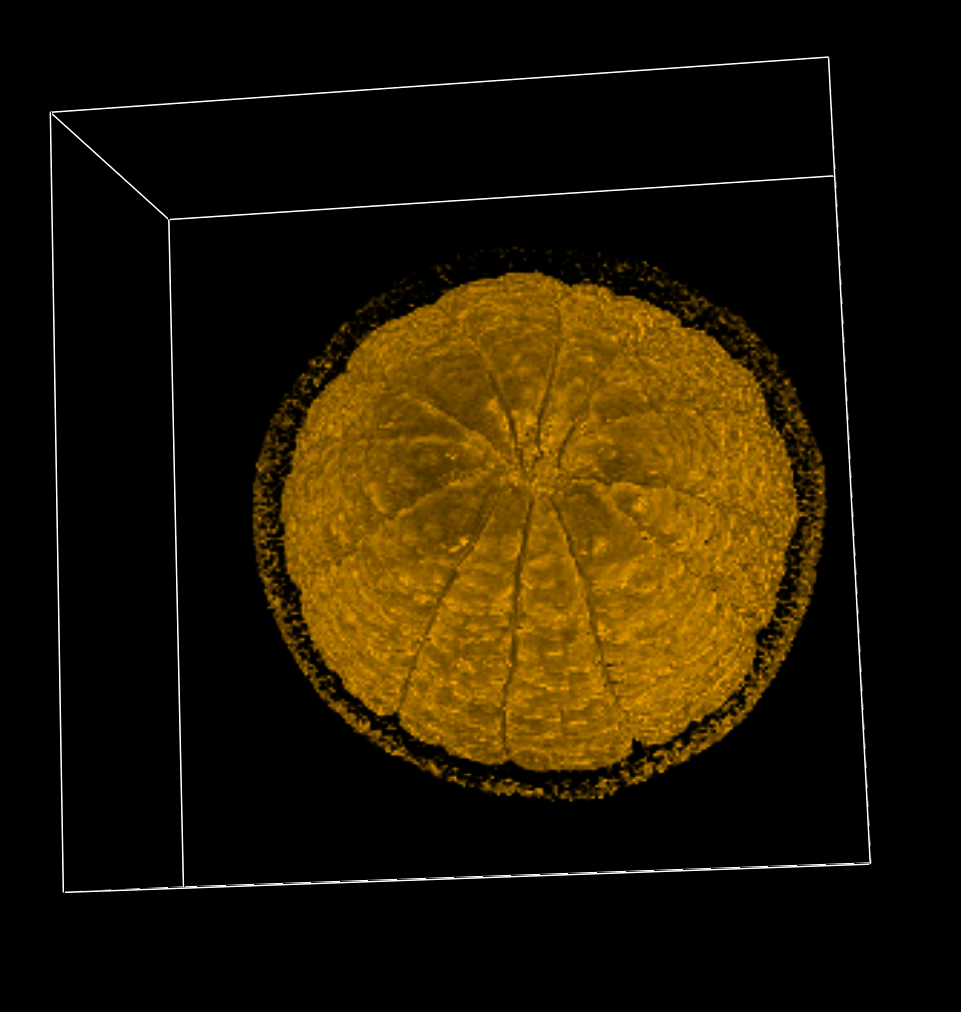
\includegraphics[width=\textwidth]{trilinear-off}
    \caption{Trilinear interpolation disabled.}
  \end{subfigure}
  \hfill
  \begin{subfigure}[b]{0.45\textwidth}
    \centering
    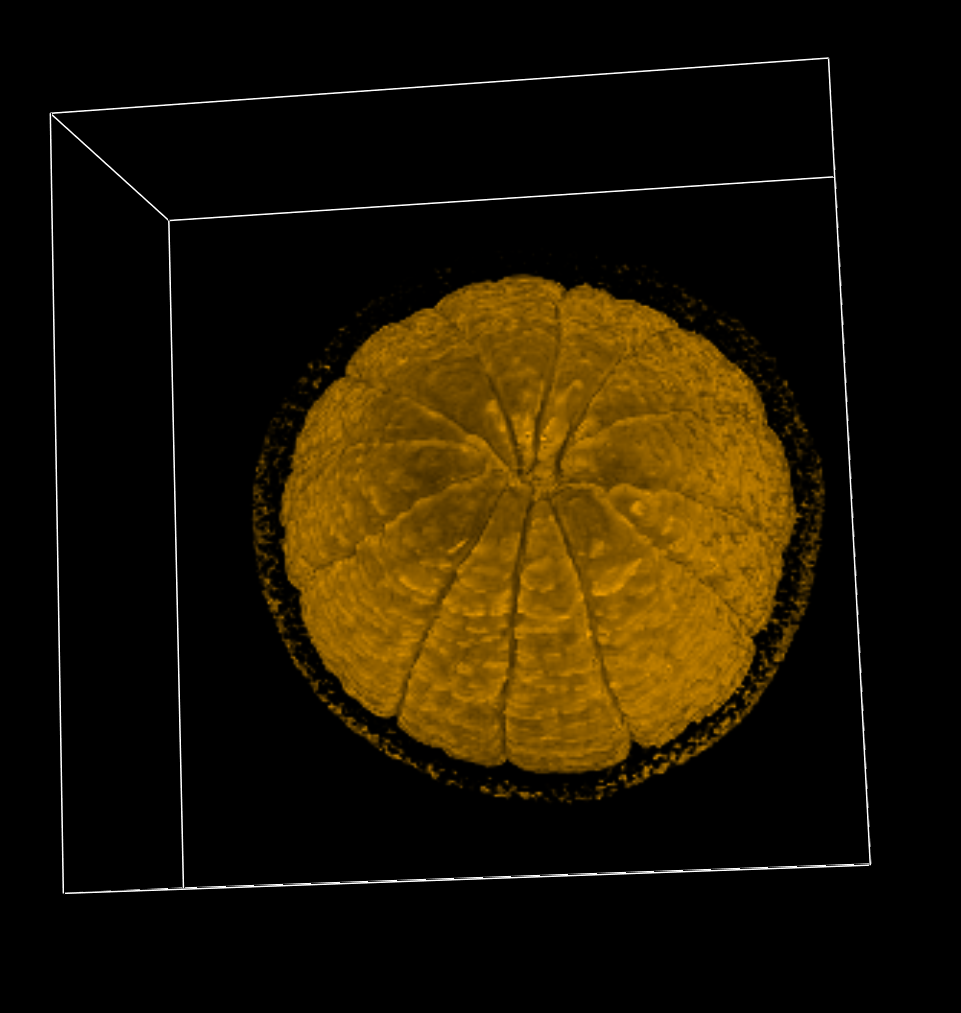
\includegraphics[width=\textwidth]{trilinear-on}
    \caption{Trilinear interpolation enabled.}
  \end{subfigure}
  \caption{Result of compositing visualization with and without trilinear interpolation on the \textit{orange} dataset.}
  \label{fig:trilinear}
\end{figure}

\begin{figure}[h]
  \centering
  \begin{subfigure}[b]{0.45\textwidth}
    \centering
    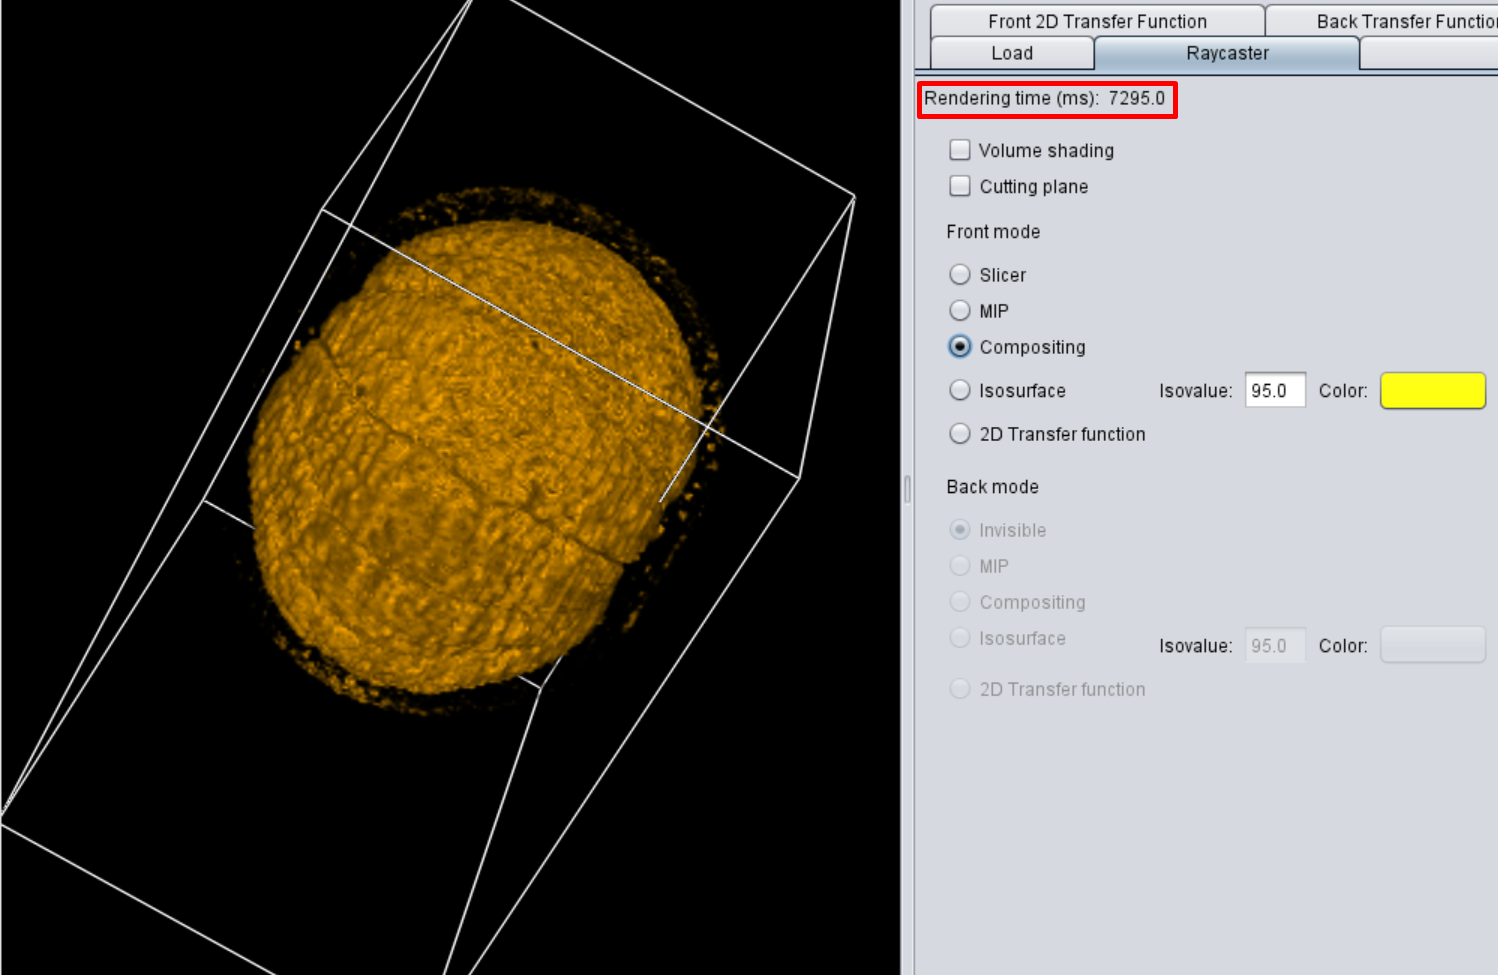
\includegraphics[width=\textwidth]{before-speedup}
    \caption{Interactive mode before speed up changes. Rendering time: 7295 ms }
  \end{subfigure}
  \hfill
  \begin{subfigure}[b]{0.45\textwidth}
    \centering
    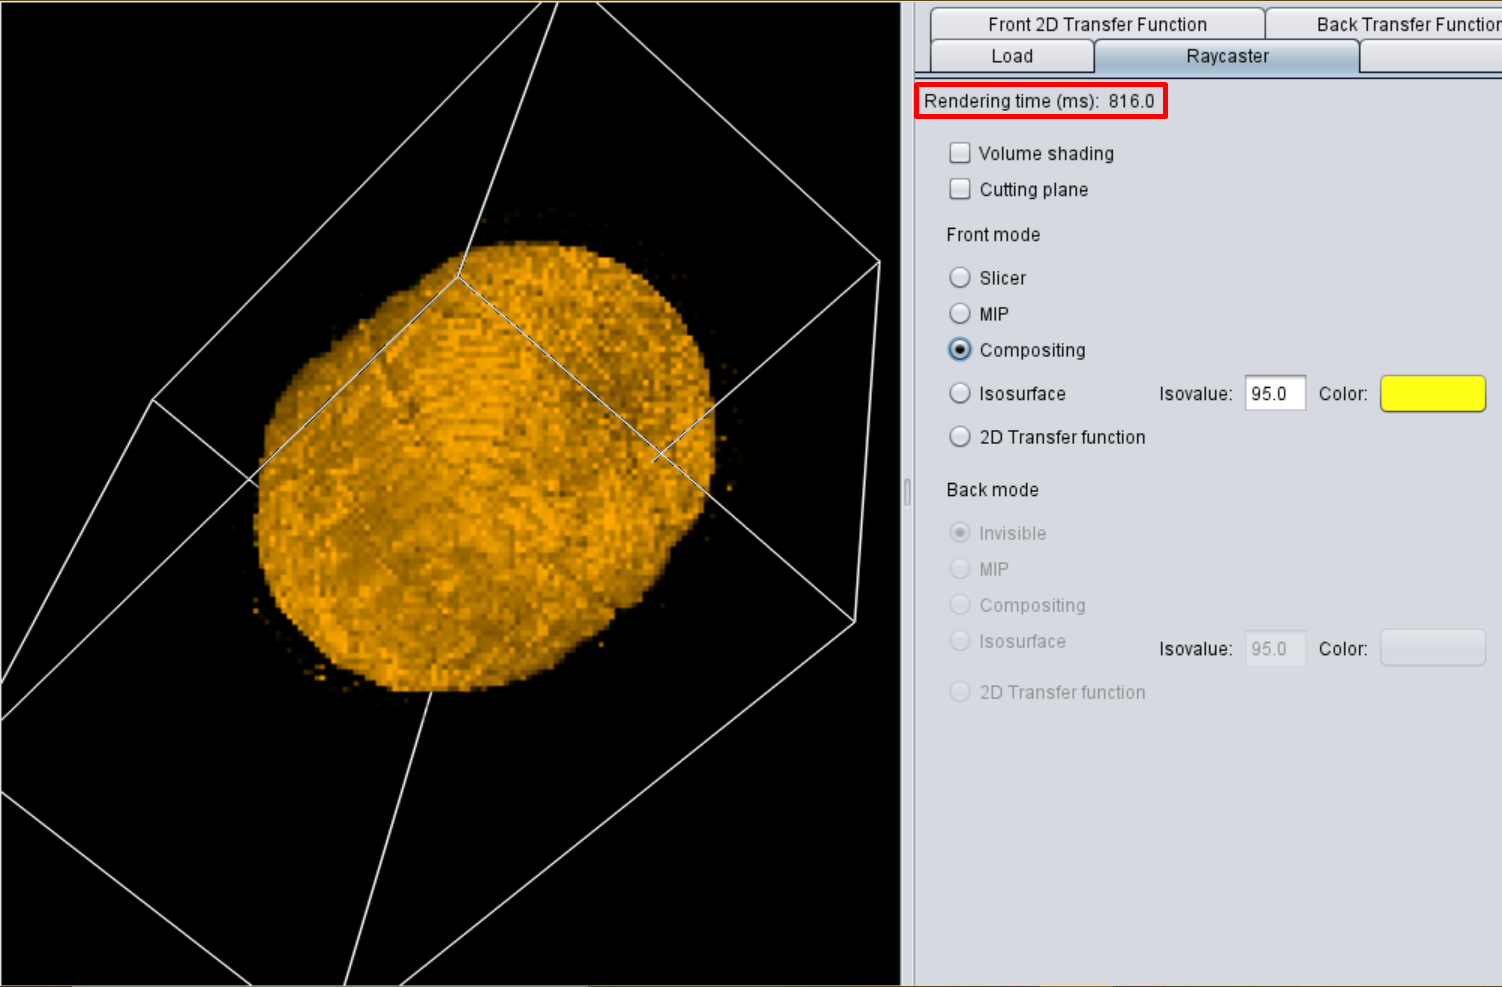
\includegraphics[width=\textwidth]{after-speedup}
    \caption{Interactive mode after speed up changes. Rendering time 816 ms}
  \end{subfigure}
  \caption{Result of speeding up interactive mode on the \textit{orange} dataset.}
  \label{fig:speedup}
\end{figure}

\begin{figure}[h]
  \centering
  \begin{subfigure}[b]{0.45\textwidth}
    \centering
    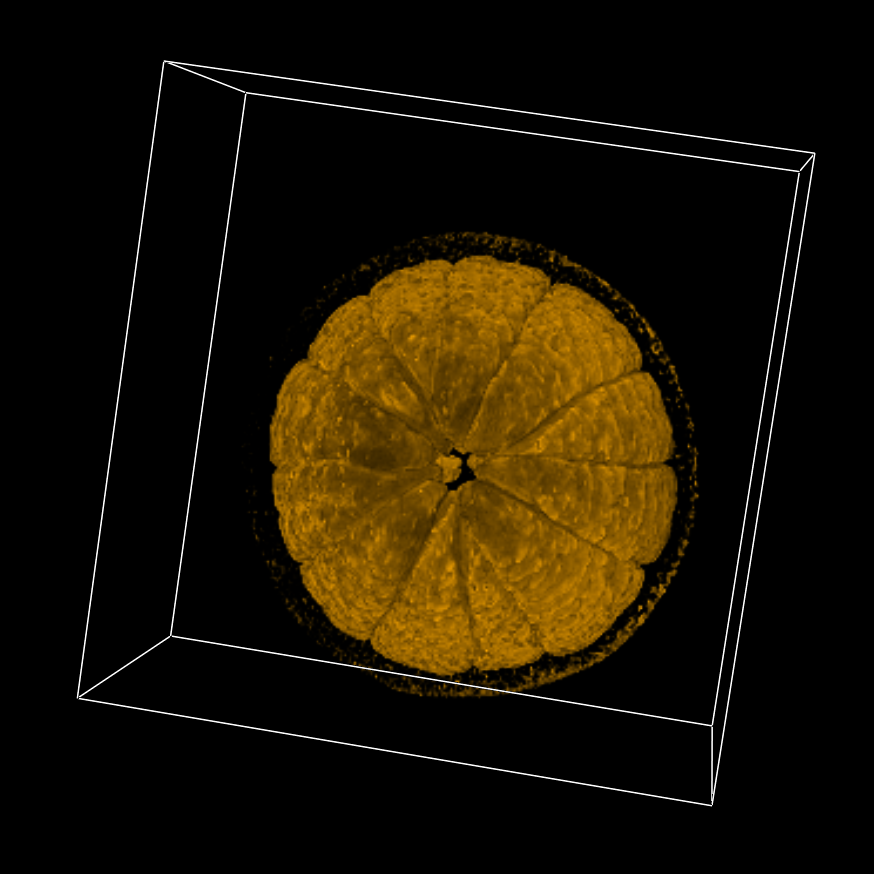
\includegraphics[width=\textwidth]{orange-composite}
    \caption{Composite with default values.}
  \end{subfigure}
  \hfill
  \begin{subfigure}[b]{0.45\textwidth}
    \centering
    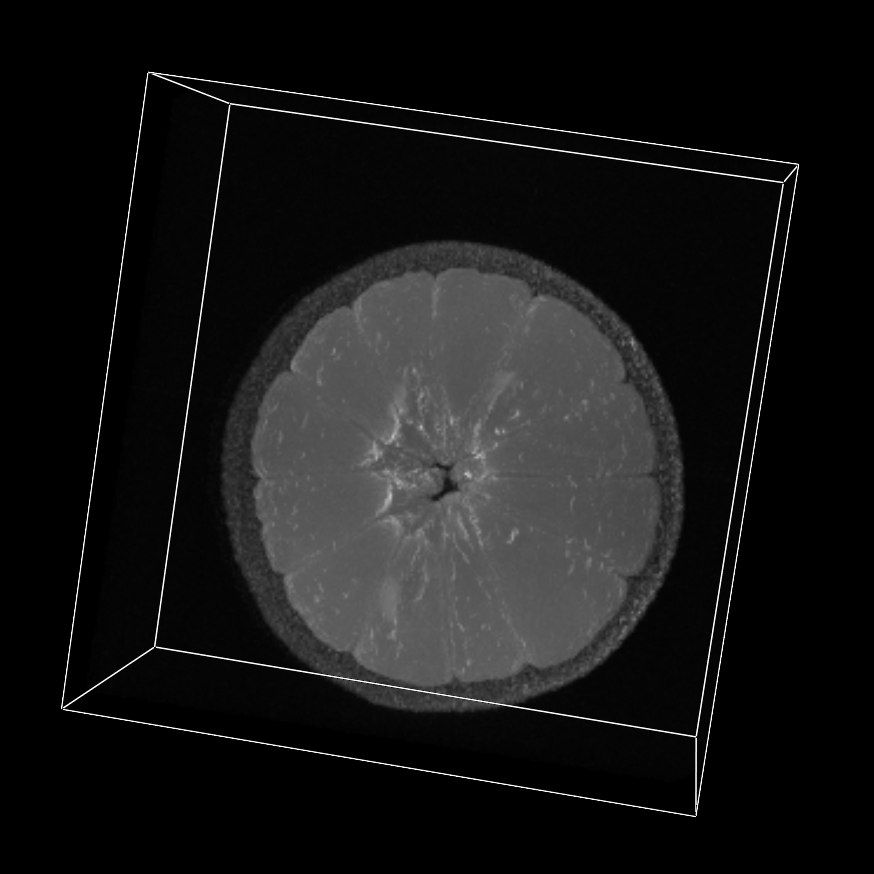
\includegraphics[width=\textwidth]{orange-mips}
    \caption{MIP with default values.}
  \end{subfigure}
  \caption{Comparison of different raycasting techniques on \textit{orange} dataset.}
  \label{fig:mipscomp}
\end{figure}

\begin{figure}[h]
  \centering
  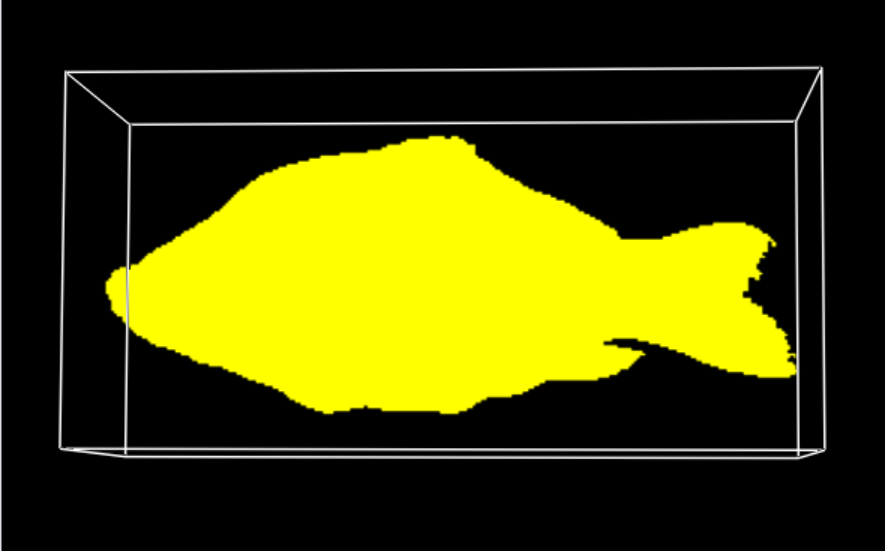
\includegraphics[width=\textwidth]{iso-surface}
  \caption{Isosurface raycasting without shading enabled on \textit{carp8} dataset.}
  \label{fig:isosurface}
\end{figure}

\begin{figure}[h]
  \centering
  \begin{subfigure}[b]{0.45\textwidth}
    \centering
    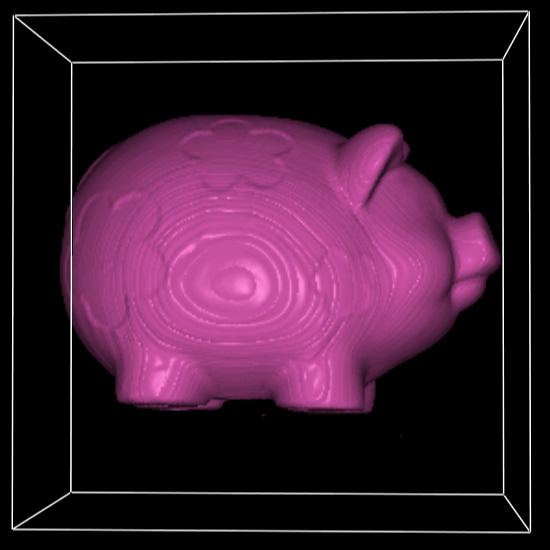
\includegraphics[width=\textwidth]{pig8-phong-default}
    \caption{Default values.}
  \end{subfigure}
  \hfill
  \begin{subfigure}[b]{0.45\textwidth}
    \centering
    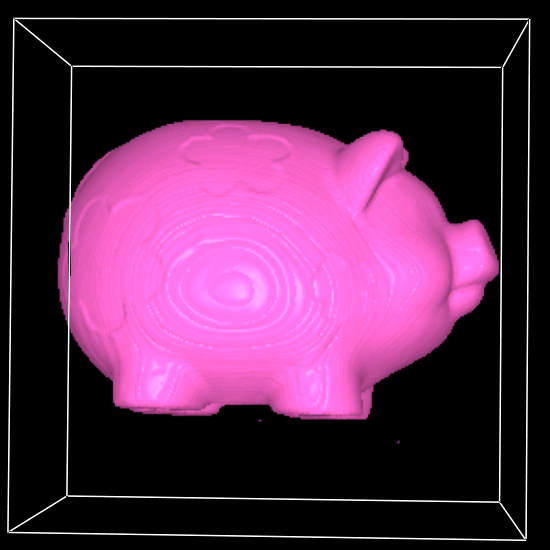
\includegraphics[width=\textwidth]{pig8-phong-ambient05}
    \caption{Ambient $k_a=0.5$, higher than the default.}
  \end{subfigure}
  \\~\\
  \begin{subfigure}[b]{0.45\textwidth}
    \centering
    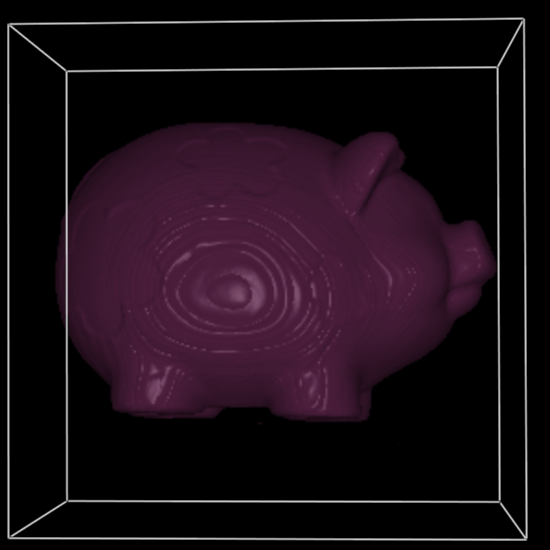
\includegraphics[width=\textwidth]{pig8-phong-diffusion02}
    \caption{Diffusion $k_d=0.2$, lower than the default.}
  \end{subfigure}
  \hfill
  \begin{subfigure}[b]{0.45\textwidth}
    \centering
    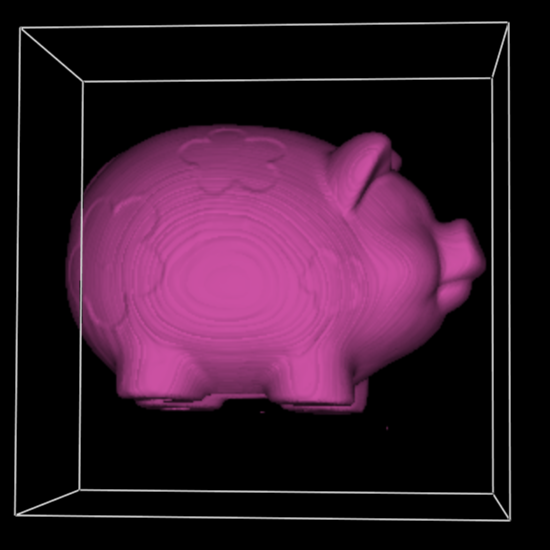
\includegraphics[width=\textwidth]{pig8-phong-specular0}
    \caption{Specular $k_s=0.0$, lower than the default.}
  \end{subfigure}
  \caption{Comparison of the effect of changing different parameters of Phong's shading on \textit{pig8} dataset.}
  \label{fig:phong}
\end{figure}


\begin{figure}[h]
  \centering
  \begin{subfigure}[b]{0.45\textwidth}
    \centering
    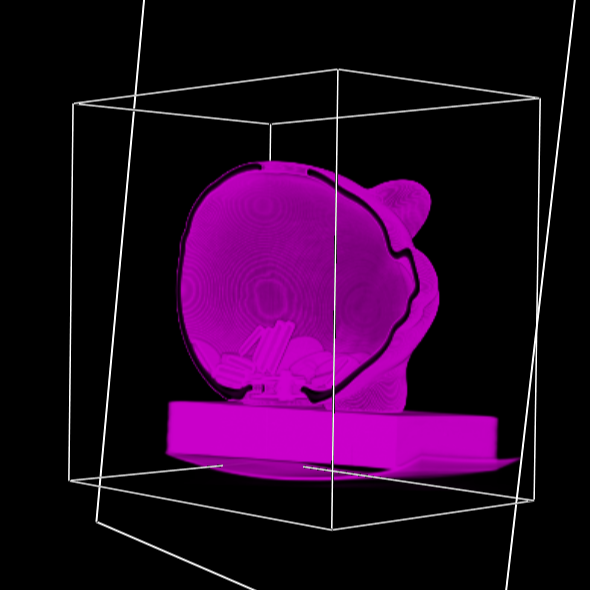
\includegraphics[width=\textwidth]{pig8-cut-plane-coins}
    \caption{Composite with cutting plane. Inside of the volume is visible.}
  \end{subfigure}
  \hfill
  \begin{subfigure}[b]{0.45\textwidth}
    \centering
    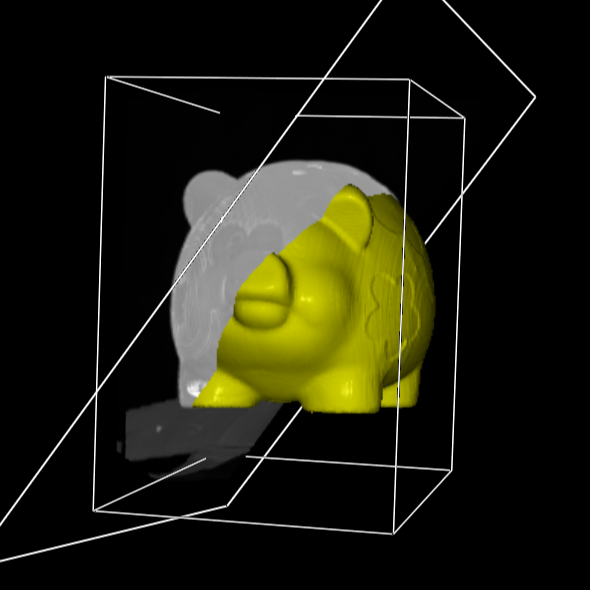
\includegraphics[width=\textwidth]{pig8-cut-plane-renders}
    \caption{MIP and Isosurface with shading. Each side of the volume is rendered differently.}
  \end{subfigure}
  \caption{Cutting plane demonstration with \textit{pig8} dataset.}
  \label{fig:cutplane}
\end{figure}

\begin{figure}[h]
  \centering
  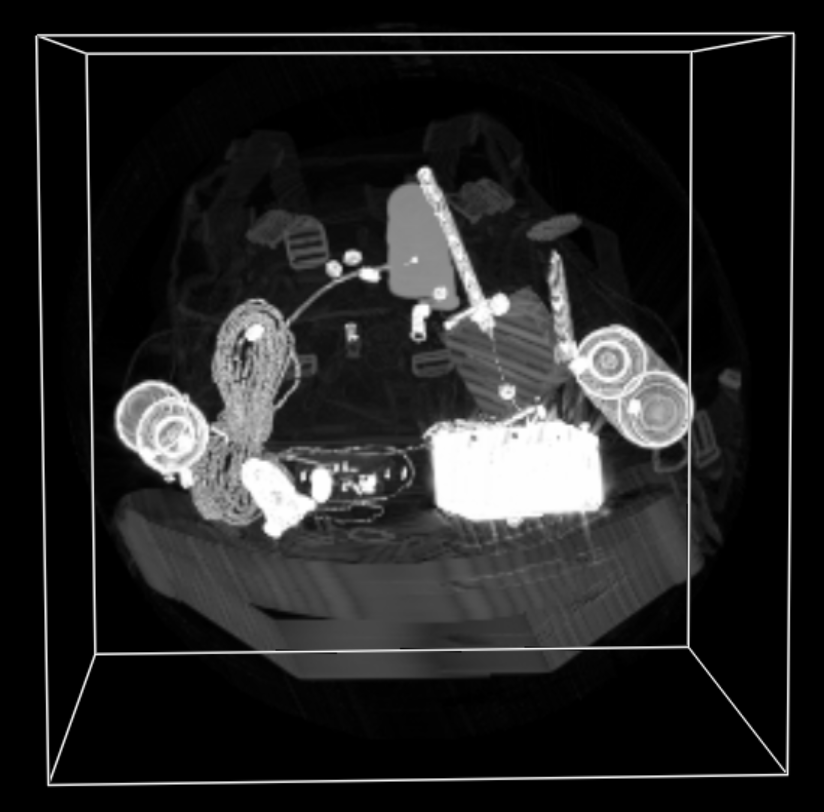
\includegraphics[width=\textwidth]{backpack-MIP}
  \caption{MIP on \textit{backpack8\_small} dataset with inside volume visible.}
  \label{fig:backpack-mip}
\end{figure}

\begin{figure}[h]
  \centering
  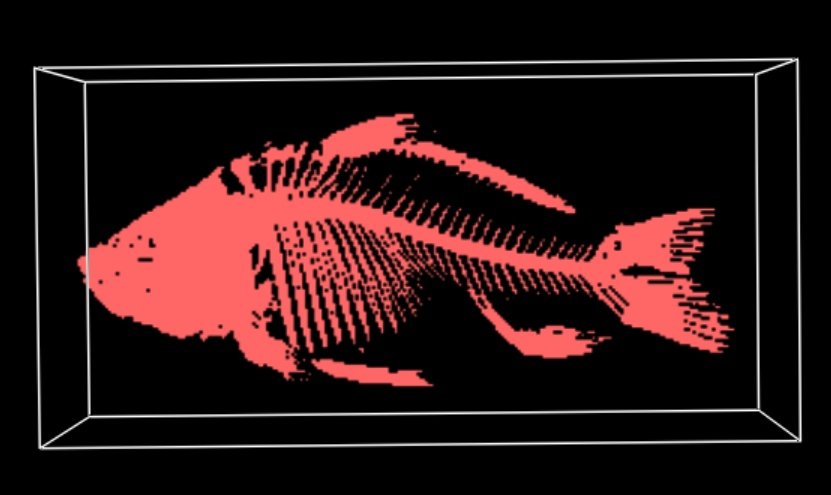
\includegraphics[width=\textwidth]{carp-iso-180}
  \caption{Isosurface raycasting with isovalue 180 on \textit{carp8} dataset.}
  \label{fig:carp-skelet}
\end{figure}

\begin{figure}[h]
  \centering
  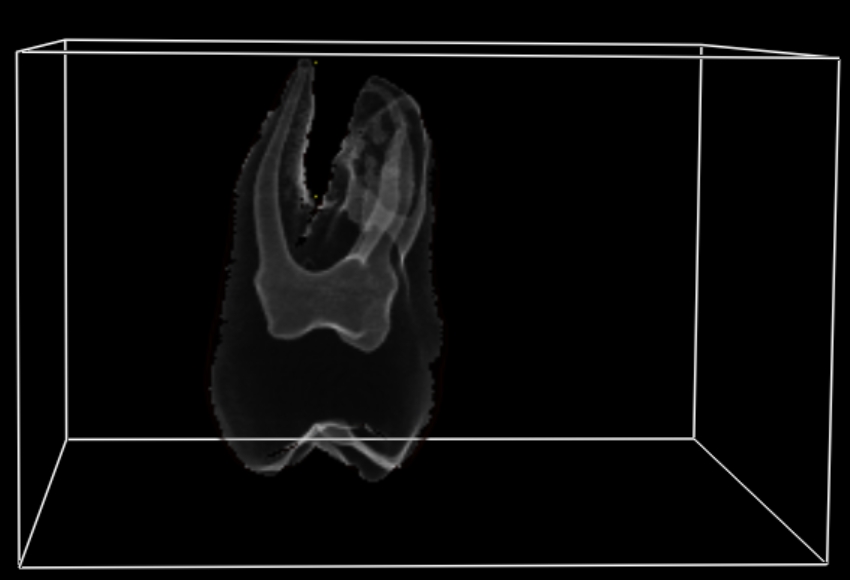
\includegraphics[width=\textwidth]{tooth-2d}
  \caption{2D transfer fuction rendering method on \textit{tooth} dataset with pulp chamber visible.}
  \label{fig:tooth}
\end{figure}

\end{document}
